\section{GNU Automake}
\begin{itemize}
	\item helps to create portable Makefiles for use with the make utility (input \textit{Makefile.am}; output \textit{Makefile.in}
	\item \textit{Makefile.in} is then used by the configure script to generate a \textit{Makefile} \cite{automake}
\end{itemize}

\begin{figure}[h!]
    \centering
    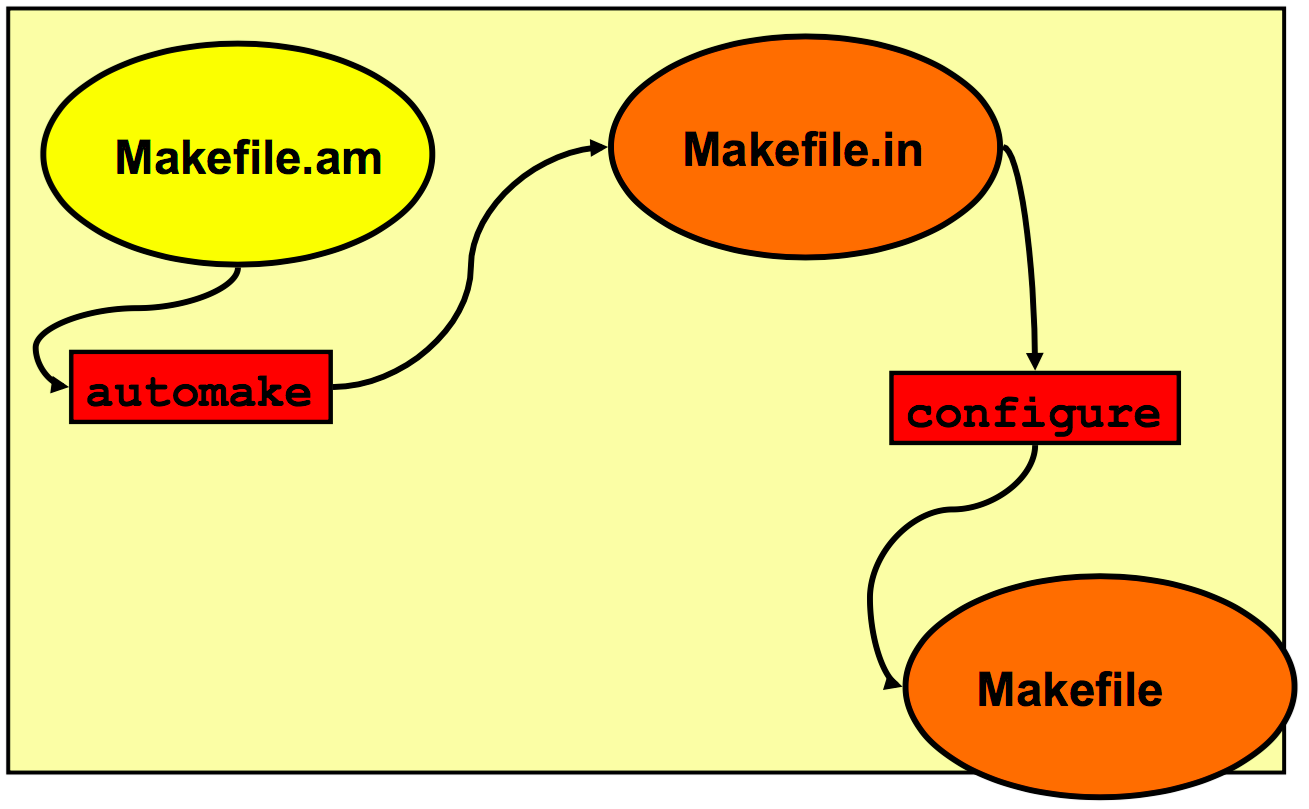
\includegraphics[width=11cm]{automake.png}
    \caption{GNU Automake procedure}
    \label{fig:automake}
\end{figure}

Usage example (as shown on the figure \ref{fig:automake}
Our package builds a program sne, simply  add the following to the \textit{Makefile.am} in the directory where the program is Built. 

Example File \textit{foo.c}
\begin{minted}{c} 
#include <stdio.h>
main()
{
	printf("Cum grano salis \n");
}
\end{minted}

File: \textit{Makefile.am}
\begin{minted}{java} 
bin_PROGRAMS = foo
foo_SOURCES = foo.c
\end{minted}


File: \textit{configure.ac}
\begin{verbatim} 
AC_INIT(foo.c)
AM_INIT_AUTOMAKE(latin_words, 0.9)
AC_PROG_CC
AC_HEADER_STDC
AC_PROG_INSTALL
AC_OUTPUT([Makefile])
\end{verbatim}

Where 
\begin{description}
	\item[AC-INIT(sourcefile)] Initializes autoconf, should be the first macro \cite{autoconf}
	\item[AM-INIT-AUTOMAKE(latin-words, 0.9)]  Runs many macros required for proper operation of the generated Makefiles
	\item[AC-PROG-CC] Determines a C compiler to use, sets the CC variable, initializes the CFLAGS
	\item[AC-HEADER-STDC] Checks for \textit{stdlib.h, stdarg.h, string.h} and \textit{float.h},  defines STDC-HEADERS on success
	\item[AC-PROG-INSTALL] Set variable INSTALL to the path of a BSD-compatible install program
	\item[AC-OUTPUT([Makefile])] Create output files in the case the Makefile.
\end{description}

\subsection{Autoheader}
\begin{itemize}
	\item Create a template header for configure 
	\item Usage ? run autoheader on a directory with a \textit{configure.ac} that contains a AC-CONFIG-HEADER macro call,  and it will write the \textit{configure.in} file 
\end{itemize}

\subsection{GNU Libtool}
\begin{itemize}
	\item helps manage the creation of static and dynamic libraries on various Unix-like operating systems
	\item hides the complexity of using shared libraries on different \cite{libtool}
\end{itemize}

\textbf{Platforms} - provide a generic interface for developers  

\begin{description}
\item[clean]  Remove files from the build directory 
\item [compile]  Compile a source file into a libtool object. 
\item [execute] AutomaMcally set the library path, then run a program. 
\item [finish]  Complete the installaMon of libtool libraries. 
\item [install]  Install libraries or executables. 
\item [link]  Create a library or an executable. 
\item [uninstall] Remove libraries from an installed directory.
\end{description}

\subsection{Steps involved in creating a software}
\begin{enumerate}
\item create source 
\item create configure.ac
\item create makefile.am
\item aclocal
\item autoconf
\item automake -a //to add missing files
\end{enumerate}



